\documentclass[12pt]{article}

\usepackage{graphicx}
\usepackage[hidelinks, colorlinks = true, urlcolor = blue, citecolor = black]{hyperref}

%opening
\title{Homework 2 - Venice Boat Classification\\
	\large Machine Learning 2018-19 - Sapienza}
\author{Luigi Russo 1699981}

\begin{document}
	
\maketitle
\newpage
\tableofcontents
\newpage
\section{Introduction}
This is my report for the second homework of Machine Learning course, about the Venice Boat Classification. First of all I will point out which have been the goals of this homework, starting of course from defining the specific classification problem (view section \ref{sec:image_classification_problem}) that I have chosen to focus on. After defining the kinds of algorithms that I have implemented and used, I will describe the dataset (view section \ref{sec:dataset}). After that, I will finally present the results of the evaluation phase (view section \ref{sec:results}).

\section{Image classification problem}
\label{sec:image_classification}
I have decided to focus on the problem of classifying \textbf{18} different classes of Venice boats. Given an instance of image, I want to be able to compute which is the correct type of boat of the input image. I have decided to use a pretrained model (Inception v3) in order to extract the features of each image: at this point, the feature vector is passed to some classifiers, such as SVM classifier. The model is then tested, computing at the end the accuracy and plotting the confusion matrix.

\subsection{Learning goals}
\subsubsection{Metrics}
The main goal of this homework is to correctly classify the input images: I will take into account both accuracy and precision metrics.
\subsubsection{Many models}
\label{sec:models}
As in the first homework, also in this one I will give great importance to the comparison between different models. Once the pretrained graph extracts the features vector of the input image, it is passed to some classifier that actually runs the last step of the classification. I have decided to compare 6 different classifiers:
\begin{itemize}
	\item Support Vector Machine (\textbf{SVM})
	\item Extra Trees (\textbf{ET})
	\item Random Forest (\textbf{RF})
	\item K-Nearest Neighbor (\textbf{KNN})
	\item Multi-Layer Perceptron (\textbf{ML})
	\item Gaussian Binomial (\textbf{GNB})
\end{itemize}

\section{Tools used}
I have used Python 3.6 programming language, because of its well-documented modules and libraries: I did not want to reinvent the wheel, so I have used the well-known \textit{Scikit-Learn}, \textit{Numpy}, \textit{Matplotlib} libraries to build, train, and evaluate the classifier. In the next sections I will give further details on the precise methods used.
I have provided the source-code as a collection of Python files (extension .py). It is possible to view the source-code in the attached zipped file (it is also present \href{https://www.gitlab.com/lrusso96/machine-learning}{in this GitLab repository}).

\section{The pretrained model}
I have decided to use Inception v3 model. In particular I have used the checkpoint of 12/05/2015, saving it in the 'pretrained' folder. This file (extension .pb) cannot be directly used, but it has to be imported, when initializing the TensorFlow session.

\section{The dataset}
\label{sec:dataset}
Both training and test images are taken from the Sapienza MarDCT dataset, a wide collection of Venice boat images. The dataset is already divided into training and test images: however, some preprocessing was needed in order to handle the different structure of the two sets of images and also because there were some multi-labeled images in the test set.

\subsection{Preprocessing}
% summary of the preprocessing phase preprocessing.py
First of all I have decided to limit the number of classes to 18 (out of the total 24), because of the number of sample images of some classes: in some cases less than 10 images. This led me to the following list of classes:
\begin{itemize}
	\item Alilaguna
	\item Ambulanza
	\item Barchino
	\item Gondola
	\item Lanciafino10m
	\item Lanciafino10mBianca
	\item Lanciafino10mMarrone
	\item Lanciamaggioredi10mBianca
	\item Motobarca
	\item Motopontonerettangolare
	\item MotoscafoACTV
	\item Mototopo
	\item Patanella
	\item Polizia
	\item Raccoltarifiuti
	\item Sandoloaremi
	\item Topa
	\item VaporettoACTV
\end{itemize}
As for the test set, it provided a ground truth text file, containing the list of all the images and their label: in some cases, however, this label was not present, or it was simply an invalid label (not present in the training set) such as multiple, partial, etc. I had to handle these issues, filtering the images with correct labels!

\subsubsection{Extract features}
Once the pretrained graph was taken into main memory from disk, they have been fed to a TensorFlow implementation of Inception v3 with the classification layer removed in order to produce a set of labeled feature vectors.

\section{Classification}
% summary of classifier.py
\subsubsection{t-sne features}
Dimensionality reduction is carried out on the 2048-D features using t-distributed stochastic neighbor embedding (\textbf{t-SNE}) to transform them into a 2-D feature which is easy to visualize. The t-SNE is used as an informative step: if the same color (i.e. label) points are mostly clustered together there is a high chance that we could use the features to train a classifier with high accuracy.

\begin{figure}[!ht]
	\centering % optional
	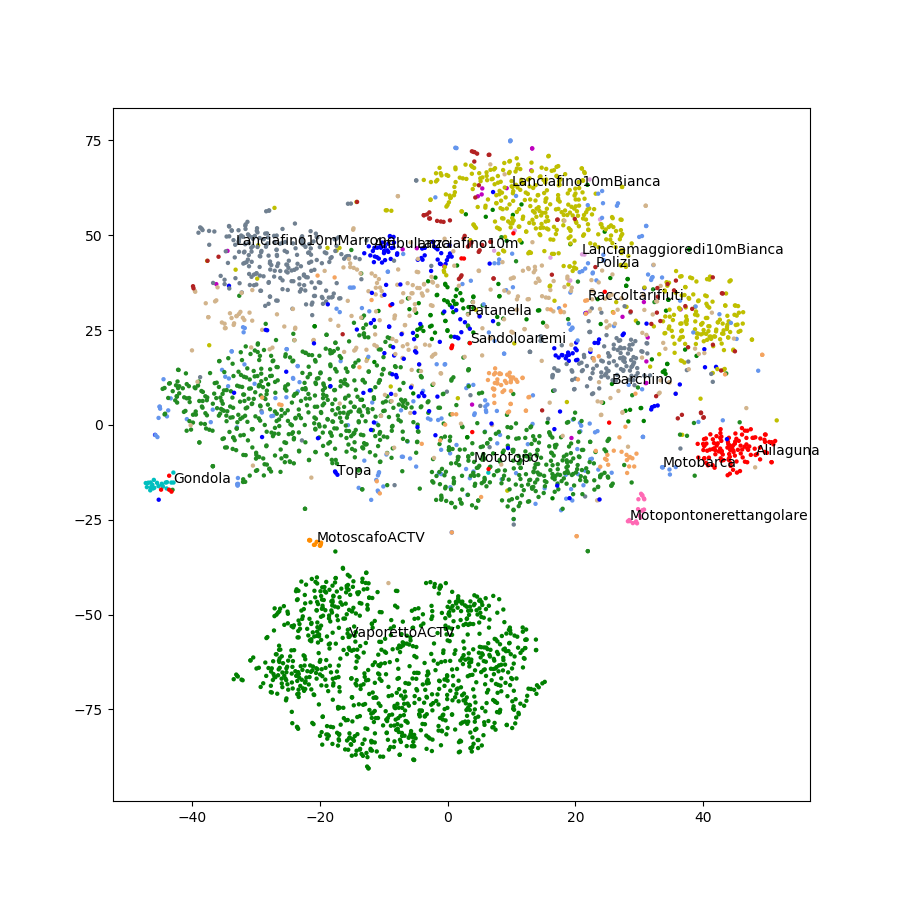
\includegraphics[width=0.7\textwidth]{../code/output/features.png} % adjust width
	\caption{\textit{t-SNE features}} % optional
	\label{fig:2dh}
\end{figure}

\subsection{Running the classifiers}
For every model (see models listed above) I have run the proper classifier: in most cases I simply used the default configuration.

\section{The results}
\label{sec:results}
\subsection{Metrics}
\begin{figure}[!ht]
	\centering % optional
	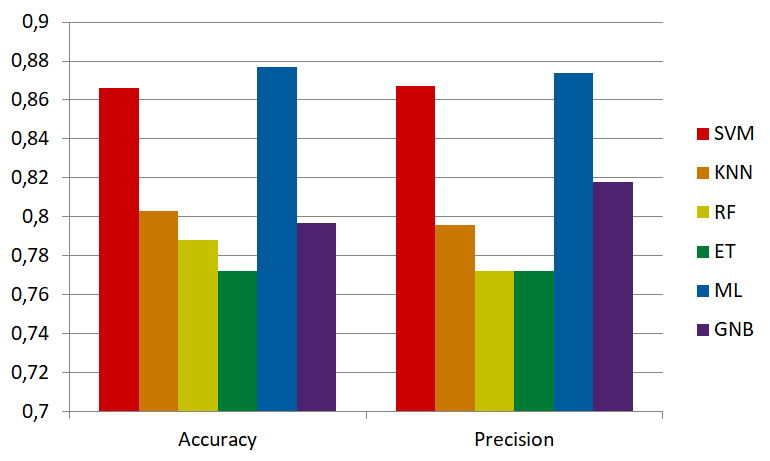
\includegraphics[width=1\textwidth]{metrics.png} % adjust width
	\caption{\textit{Precision and accuracy of the classifiers}} % optional
	\label{fig:metrics}
\end{figure}
\subsubsection{SVM}
The accuracy was 86.6\% and the precision was 86.7\%
\subsubsection{KNN}
The accuracy was 80.3\% and the precision was 79.6\%
\subsubsection{RF}
The accuracy was 78.8\% and the precision was 77.2\%
\subsubsection{ET}
The accuracy was 77.2\% and the precision was 77.2\%
\subsubsection{ML}
The accuracy was 87.7\% and the precision was 87.4\%
\subsubsection{GNB}
The accuracy was 79.7\% and the precision was 81.8\%


\subsection{Confusion matrices}
For each model I have also plotted the confusion matrix (not normalized!). They are shown in the following images.

\begin{figure}[!ht]
	\centering
	\begin{minipage}{.5\textwidth}
		\centering
		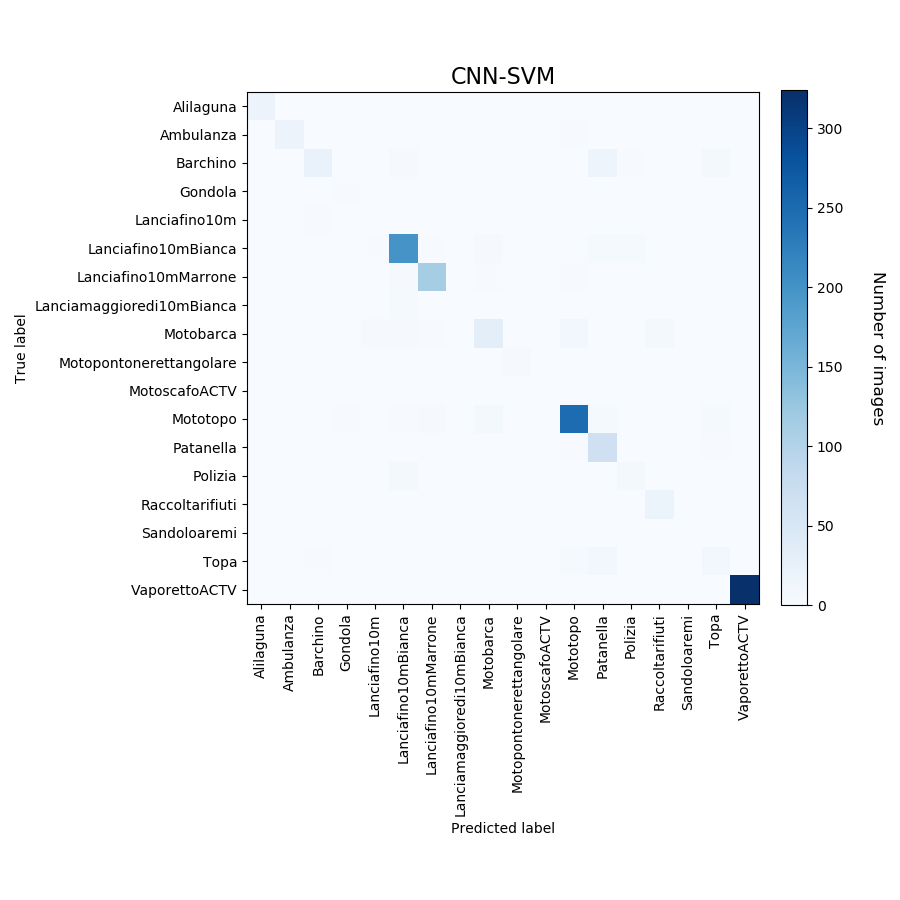
\includegraphics[width=.8\linewidth]{../code/output/CNN-SVM.png}
		\caption{SVM confusion matrix} % optional
		\label{fig:cnf_svm}
	\end{minipage}%
	\begin{minipage}{.5\textwidth}
		\centering
		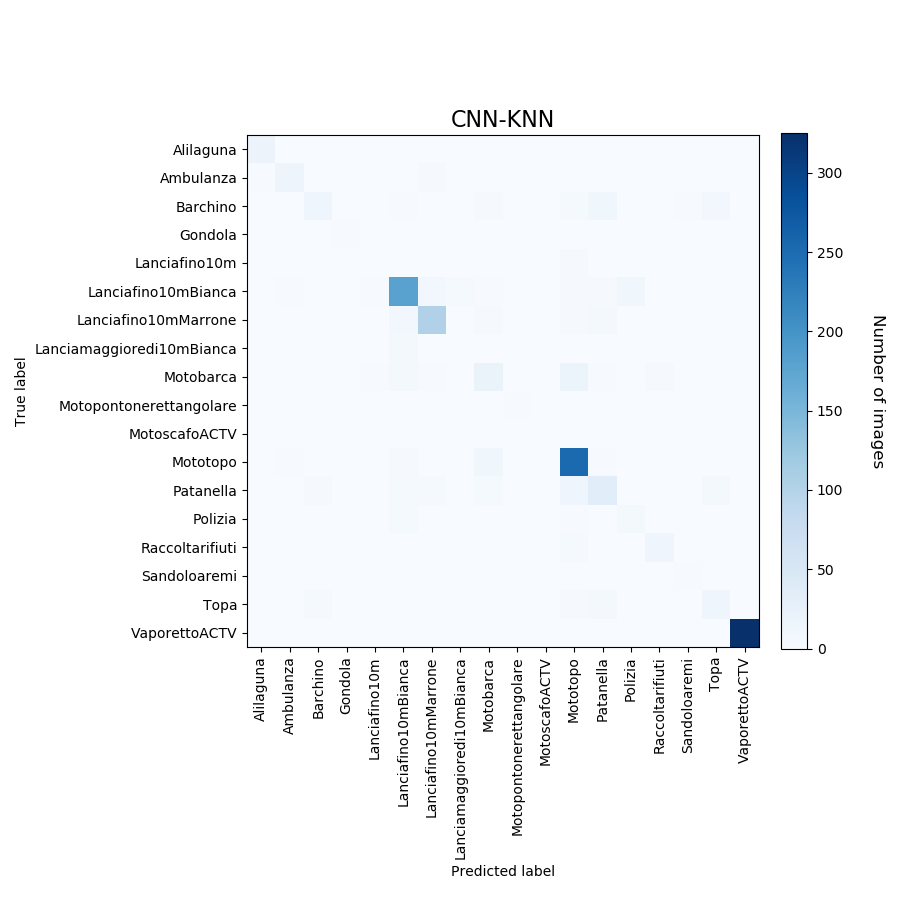
\includegraphics[width=.8\linewidth]{../code/output/CNN-KNN.png}
		\caption{KNN confusion matrix} % optional
		\label{fig:cnf_knn}
	\end{minipage}
\end{figure}
\begin{figure}[!ht]
	\centering
	\begin{minipage}{.5\textwidth}
		\centering
		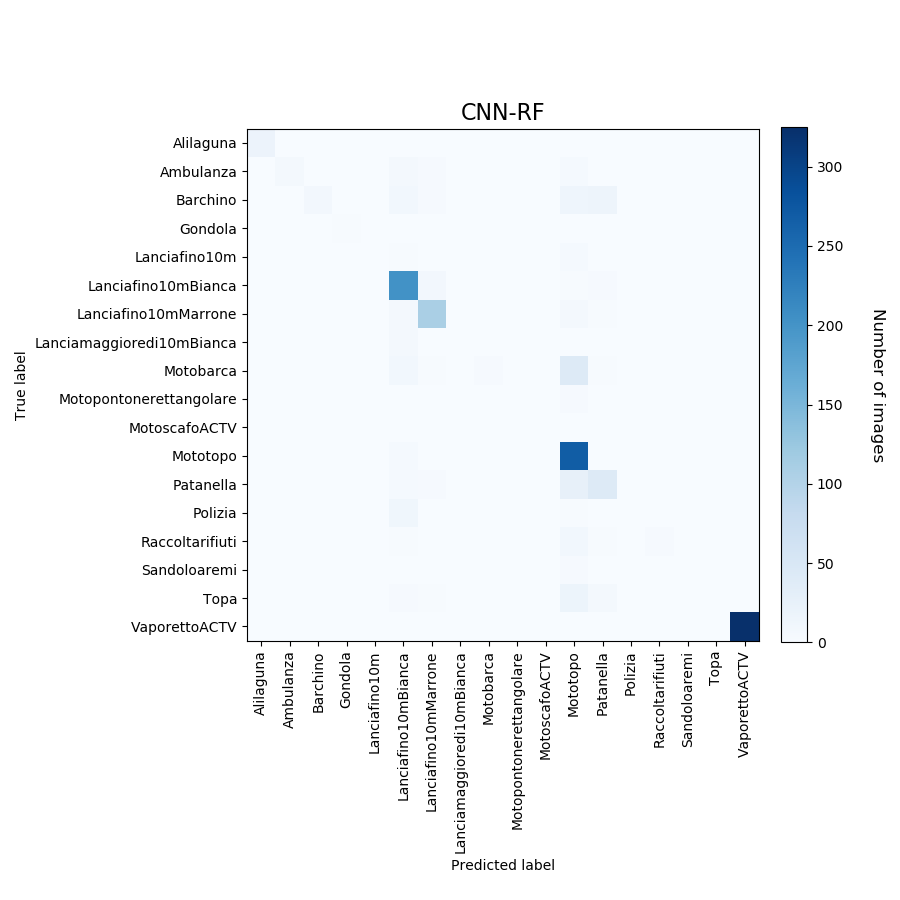
\includegraphics[width=.8\linewidth]{../code/output/CNN-RF.png}
		\caption{RF confusion matrix} % optional
		\label{fig:cnf_rf}
	\end{minipage}%
	\begin{minipage}{.5\textwidth}
		\centering
		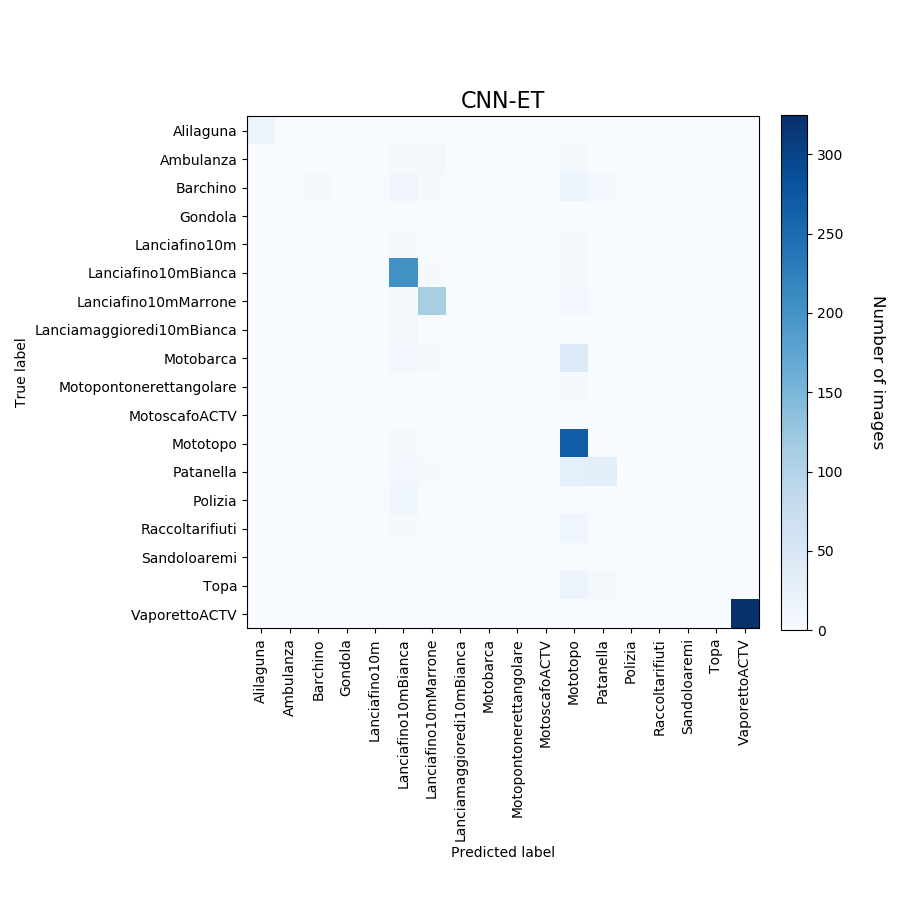
\includegraphics[width=.8\linewidth]{../code/output/CNN-ET.png}
		\caption{ET confusion matrix} % optional
		\label{fig:cnf_et}
	\end{minipage}
\end{figure}
\begin{figure}[!ht]
	\centering
	\begin{minipage}{.5\textwidth}
		\centering
		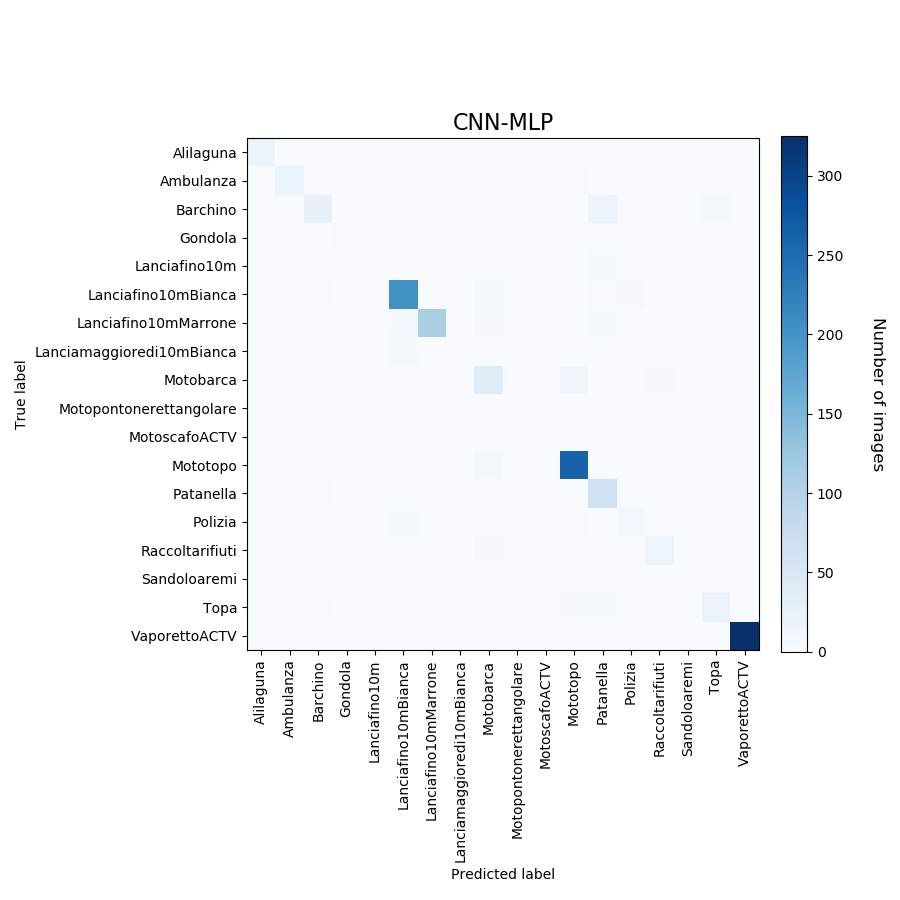
\includegraphics[width=.8\linewidth]{../code/output/CNN-MLP.png}
		\caption{ML confusion matrix} % optional
		\label{fig:cnf_mlp}
	\end{minipage}%
	\begin{minipage}{.5\textwidth}
		\centering
		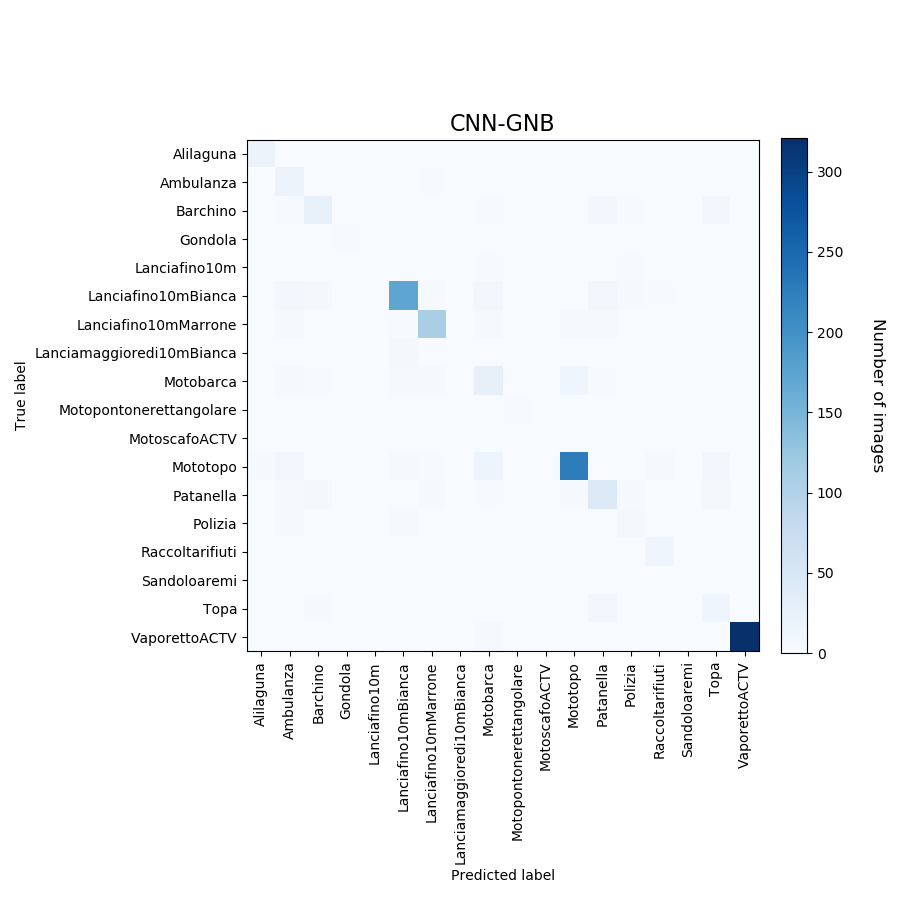
\includegraphics[width=.8\linewidth]{../code/output/CNN-GNB.png}
		\caption{GNB confusion matrix} % optional
		\label{fig:cnf_gnb}
	\end{minipage}
\end{figure}

\section{Conclusions}
The model with highest accuracy and precision is the Gaussian Binomial.

\newpage
\begin{thebibliography}{10}
	
	% bibitem for book
	\bibitem{Main Book}
	Tom M. Mitchell \textsl{Machine Learning}.
	
\end{thebibliography}
\end{document}